\section{Privacy and Data Protection}
\subsection{Privacy}
With the term privacy we refers to two concepts: at first privacy means that everyone gets to \textbf{control} information about herself/himself, so the owner decide who can access his data (like we do everyday with cookies). Privacy means also the requirement of high-level of difficulty in \textbf{correlating} data/actions, this definition is more related to the possibility of remaning anonymous online, this can considered a difficoult task because we don't always want to be able to be anonymous online. 

As we can immagine the notion of privacy is high correlated with what we have saw for the security techniques.
\begin{figure}[h!]
    \centering
    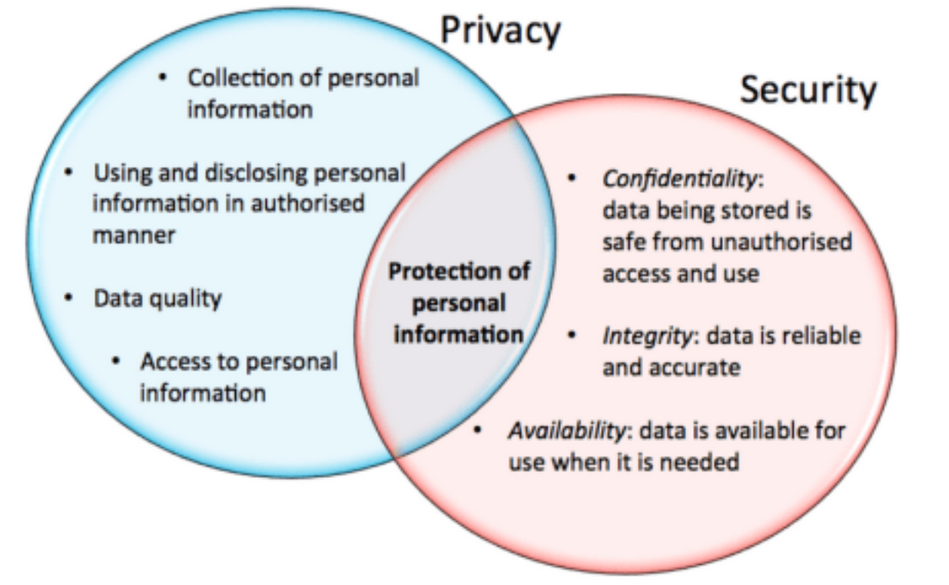
\includegraphics[scale=0.35]{images/privacy1.png}
\end{figure}

\FloatBarrier

For example we can use the techniques for ensuring confidentiality for guaranting that our personal data are shared only at the ones that we trust, integrity and availability are used to guarantee fondamental rights in freedom.

\myparagraph{LINDDUN}
Is an acronym that characterize the notion of privacy.
\begin{itemize}
    \item \textbf{Linkability}: Being able to sufficently distinguish whether two \textbf{items of interest (ioi)} are linked or not, even without knowing the actual identity of the subject of the linkable ioi (e.g. entries in database related to tge same person). If violated you become more \textbf{Identifiable} and subject of \textbf{inference} (when "group data" is linkable, this can lead to societal harm, like discrimination).  
    \item \textbf{Identifiability}: Being able to sufficently identify the subject within a set of subjects, is related to the notion of digital identity (e.g. identifing the person to whom an entry in a database relates). This leads to severe privacy violations cause the subject assumes he is anonymous.
    \item \textbf{Non-repudiation}: Not being able to dany a claim, when a person is not able to repudiate an action or piece of information, he can be held accountable.
    \item \textbf{Detectability}: being able to sufficently distinguish whether an ioi exists or not, by detecting whether an ioi exists, one can deduce certain information, even without actually having access to that information.
    \item \textbf{Disclosure of information}: Related to violation of confidentiality and thus more to security
    \item \textbf{Unawareness}: Being unaware of the consequences of sharing information, often users are not aware of the impact of sharing data like photos online ecc but also personal information shared with other services. Ideally all users should be clearly informed and educated of the consequences of sharing data. Remember, the more information is available, the easier it can be linked.
    \item \textbf{Non-compliance}: Not being compliant with legislation, regulations and corporate policies. This leads to fines and loss of image and credibility.
\end{itemize}

The first five proprieties are mainly enfored with technology such as cryptography and other technique that we have seen, the las two proprieties are the so called \textbf{soft privacy}, there is no way to enforce these with technology, only an human aspect.

\subsection{Anonymization}
When performing data anonymization we refer to the process of removing Personally Identifying Information (\textbf{PII}) like Name, Social security number, phone number ecc. But this has no technical meaning, it isn't a math thing, in orivacy breaches, any information can be personally identifying such as the Netflix Prize dataset.

\myparagraph{Netflix Data Leak}
In 2006 Netflix launched the netflix price, the goal was to improve movie recommendations algorithm of at least 10\%, for testing Netflix released 100 milion supposedly anonymized movie ratings, each included unique subscriber ID, the movie title, year of release and the date on which the subscriber rated the movie. Just 16 days later two universities researchers annouced that they had identified some of the netflix users in the dataset, they where able to identify targets by matching their Netflix reviews with data from other sites like IMDb.
\\\\
This descripted is the so called \textbf{Linkage attack}, attackers learns sensitive data by joining two datasets on common attributes or demographic attributes. They usually use the \textbf{Quasi-identifiers}, are the attributes like the ZIP code, birth date or the gender, they uniquely identifies 63\% of US popolation nowadays. Publishing a record with a Quasi-identifier is as bad as publishing it with an explicit identity.

A common used mitigation for these types of attacks is the \textbf{k-anonymity}: the information for each person contained in the released table cannot be distingushed from at least k-1 individuals whose information also appears in the release (to be more practice there are k men in the table with the same birth date and gender). Any quasi-identifier present in the released table must appear in at least k records.

Another method used is the \textbf{generalization}: replace quasi-identifiers with less specific but semantically consistent values until get k identical, example all the age from 20 to 29 are now 2*.

\myparagraph{Pseudonymization functions}
A pseudonymization function maps identifiers to pseudonyms:
\begin{itemize}
    \item \textbf{Counter}: Identifiers are substituted by a number chosen by a monotonic counter, a seed s is set to 0 (for instance) and then is incremented, values oriduced by the counter never repeat to prevent any ambiguity. Is a very simple mechanism but sequential character of the counter can orovide information on the order of the data.
    \item \textbf{Pseudo Random Number Generator}: Similar to counter although more complex solution, difficoult to implement (avoid repetitions) but no sequential issue.
    \item \textbf{Cryptographic Hash Function}: The digest of the identifiers is the pseudonym, it is considered inadequate for pseudonymization as it is prone to brute force and dictionary attacks.
    \item \textbf{Encryption}: Usually block ciphers like the AES are used for pseudonymization, the block cipher is used to encrypt an identifier using a secret key, which is both the pseudonymisation and recovery secret.
\end{itemize}       

\subsection{GDPR}
Data privacy laws and regulations vary from country to country and even from state to state, the European Union's General Data Protection Regulation (\textbf{GDPR}) went into effect in May, 25 2018. Compliance with any one set of rules is complicated and challenging, GDPR is applyed  to every european citizen, this has effect also to company not based mainly in europe (like Google). It's a regulation, is applied to all in the same manner, other countries cannot modify it. The aim of GDPR is to minimize the abuse of personal information since most of OTT business is around abusing personal information (like Meta). 


The main entity for GDPR is the 
\textbf{Data controller}: entity that offer service and has responsability to perform the data process activity compliant to regulation, it may use \textbf{data processor}, are usually IT companies that provide pieces for app/service to process personal data, it has to setup a contract that guarantee that is done in the appropriate way. Before performing data processing a \textbf{data privacy impact analisis} has to be performed, this is done to ensure that data processing activity do not collect much personal information, or better, collect minimal personal data needed. This is similar to the least privilege principle.

\myparagraph{Some articles from GDPR}
\begin{itemize}
    \item \textbf{Art 4: Definitions}
    \begin{itemize}
        \item \textbf{Personal data}: means any information relating to an identified or identifiable natural person.
        \item \textbf{Processing}: means any operation or set of operations which is performed on personal data or on sets of personal data.
        \item \textbf{Pseudonymisation}: means the processing of personal data in such a manner that the personal data can no longer be attributed to a specific data subject without the use of additional information.
        \item \textbf{Controller}: means the natural or legal person, public authority, agency or other body which, alone or jointly with others, determines the purposes and means of the processing of personal data.
        \item \textbf{Processor}: means a natural or legal person, public authority, agency or other body which processes personal data on behalf of the controller.
        \item \textbf{Consent} of the data subject means any freely given, specific, informed and unambuguous indication of the data subject's wishes by which he or she, by a statement or by a clear affermative action, signifies agreement to the processing of personal data relating to him or her.
        \item \textbf{Personal data breach}: means a breach of security leading to the accidental or unlawful destruction, loss, alteration, unauthorized disclosure of, or access to, personal data transmitted, stored or otherwise processed.
    \end{itemize}
    \item \textbf{Art. 7: Conditions for consent}
    \\ Where processing is based on consent, the controller shall be able to demonstrate that the data subject \textbf{has consented} to processing of his or her personal data. If the data subject's consent is given in the context of a written declaration which also concerns other matters, the request for consent shall be presented in a manner which is clearly distinguishable from the other matters, in an intelligible and easily accessible form, using clear and plain language. The data subject \textbf{shall have the right} to withdraw his or her consent at any time.
    \item \textbf{Art. 32: Security of processing}
    \\ The controller and the processor shall implement appropriate (state of art) technical and organisational measures to ensure a level of security appropriate to the risk, including inter alia as appropriate: the pseudonymization and encryption of personal data, the ability to ensure the ongoing confidentiality, integrity and availability and resilience of processing systems and services (this is very general). In assessing the appropriate level of security account shall be takenin particular of the risks that are presented by processing.
    \item \textbf{Art. 33: Notification of a personal data breach to the supervisory authority}
    \\ In the case of a personal data breach the controller shall without undue delay and, where feasible, not later than 72 hours after having become aware of it, notify the personal data breach to the supervisory authority competent unless the personal data breach is unlikely to result in a risk to the rights and freedoms of natural persons. The processor shall notify the controller without undue delay after becoming aware of a personal data breach.
    \item \textbf{Art. 34: Communication of a personal data breach to the data subject}
    \\ When the personal data breach is likely to result in high risk to the rights and freedoms of natural persons, the controller shall communicate the personal data breach to the data subject without undue delay.
    \item \textbf{Art. 35: Data protection impact assessment}
    \\ Where a type of processing in particular using new technologies, and taking into account the nature, scope, context and purposes of the processing, is likely to result in a high risk to the rights and freedoms of natural persons, the controller shall, prior to the processing, carry out an assessment of the impact of the envisaged processing operations on the protection of personal data.
    The assessment shall contain at least: a systematic description of the envisaged processing operations and the purposes of the processing, an assessment of the risks to the rights and freedoms of data subjects. 
\end{itemize}
